\PassOptionsToPackage{offset}{pdfpcnotes}

\documentclass[
% auto_overview,
auto_sections,
% show_durations,
monitor_progress,
draft
]{mannbeamer}

\setkeys{Gin}{draft=false}

\usepackage[utf8]{inputenc}
\usepackage[T1]{fontenc}

\usepackage{default}

\usetikzlibrary{arrows,arrows.meta,calc,positioning,shapes,decorations.pathreplacing,decorations.markings}

\setbeamertemplate{caption}{\raggedright\insertcaption\par}

\usepackage[backend=biber,maxcitenames=1,doi=false,isbn=false,url=false]{biblatex}
\addbibresource{thesis.bib}

% Complex arrays with diagonal headers
\usepackage{booktabs}
\usepackage{adjustbox}
\usepackage{array}
\usepackage{multirow}

\usepackage{multimedia}

\usepackage{amsmath}

\usepackage{qrcode}

\let\vec\mathbf

% Seems to work. But I'm really not sure.
\AtDataInput{%
  \stepcounter{citations}
}

\DeclareCiteCommand{\citejournal}
  {\usebibmacro{prenote}}
  {\usebibmacro{citeindex}\usebibmacro{journal}}
  {\multicitedelim}
  {\usebibmacro{postnote}}
\newcommand{\mycite}[2][\tiny]{\stepcounter{citations}{#1\citeauthor{#2} \citeyear{#2} - \citejournal{#2}}}
\newcommand{\mysmallcite}[2][\tiny]{\stepcounter{citations}{#1\citeauthor{#2} (\citeyear{#2})}}

\graphicspath{{annexes/}{annexes_slides/}}

\titleheader{
 \includegraphics[height=1.5cm]{logos/IRIT}
 \hfill
 \includegraphics[height=1.5cm]{logos/REVA}
 \hfill
 \includegraphics[height=1.5cm]{logos/UTMP}
}
\title{Splinoids project outline}
\author{GODIN-DUBOIS Kevin}
% \formation{Background}
\date{March 31st, 2020}
\duration{8}
\notessize{30}

\begin{document}

\dotitlepage

\newcommand{\splinoid}[2][]{\includegraphics[draft=false,#1]{splinoids_#2.png}}
\section{Splinoids}

\begin{frame}[ok]
 \frametitle{Spline + Boids}
 \centering
 \begin{minipage}{.49\textwidth}
  \splinoid[width=\textwidth, height=.8\textheight, keepaspectratio]{large}
 \end{minipage}
 \begin{minipage}{.49\textwidth}
  \begin{itemize}
   \item 2D creatures
   \item Low-level combat
   \item Low-level vision
   \item Growth
   \item Autonomous reproduction
   \item Sexual dimorphism
  \end{itemize}
 \end{minipage}
\end{frame}

\subsection{Anatomy}
\begin{frame}[ok]
 \centering
 \newlength{\imagewidth}
 \settowidth{\imagewidth}{\splinoid{anatomy}}
 \resizebox{\textwidth}{!}{
 \begin{tikzpicture}
  \node (SL)
   [inner sep=0pt]
   {\splinoid[trim=0 0 .5\imagewidth{} 0, clip, height=.8\textheight]{anatomy}};
   
  \node (SR)
   [right=0 of SL, inner sep=0pt]
   {\splinoid[trim=.5\imagewidth{} 0 0 0, clip, height=.8\textheight]{anatomy_wireframe}};
   
  \node (s) at (SL.north west)
   {\setlength{\tabcolsep}{0pt}\begin{tabular}{c}Artifacts\\\small\emph{(Bezier Curves)}\end{tabular}};
  \draw [dotted] (s) -- ($(SL.north west)+(3,-.5)$);
  \draw [dotted] (s) -- ($(SL.north west)+(.8,-1.6)$);

  \node (i) at (SL.south west) [anchor=south west]
   {\setlength{\tabcolsep}{0pt}\begin{tabular}{c}Inactive\\artifacts\end{tabular}};
  \draw [dotted] (i) -- ($(SL.south west)+(3,4)$);
  \draw [dotted] (i) -- ($(SL.south west)+(3,3)$);
  
  \node (b) at (SR.south east) [anchor=south east] {Fragile body};
  \draw [dotted] (b) -- ++(-1, 1);
  
  \node (a) at (SR.north east)
   {\setlength{\tabcolsep}{0pt}\begin{tabular}{c}Simplified splines\\\small\emph{for physics}\end{tabular}};
  \draw [dotted] (a) -- ($(SR.north east)-(3,.5)$);
  \draw [dotted] (a) -- ($(SR.north east)-(.8,1.6)$);
 \end{tikzpicture}
 }
\end{frame}

\subsection{Combat}
\begin{frame}[ok]
 \begin{itemize}
  \item Based on physical collision of primitives
  \item Both creatures receive damage\footnote{Unlike \cite{Miconi2008b}}
  \item Artifacts are denser and more resilient than the body
  \item Health regenerates but is costly
 \end{itemize}
\end{frame}

\subsection{Motion}
\begin{frame}[hok]
 \begin{minipage}{.59\textwidth}
 \centering
 \begin{tikzpicture}
  \node [inner sep=0pt] (S) {\splinoid[height=.5\textheight]{motors}};
  \begin{localto}{S}
   \node (l) at (S.north) [anchor=south] {\setlength{\tabcolsep}{0pt}\begin{tabular}{c}Motors\\$\in [-1,1]$\end{tabular}};
   \draw [dotted] (l) -| (-.32, 0) (l) -| (.32, 0);
  \end{localto}
 \end{tikzpicture}
 \end{minipage}
 \begin{minipage}{.39\textwidth}
  Tank-like behavior:
  
  \begin{tabular}{@{\{}r@{,}r@{\} $\rightarrow$ }l}
    1 &  1 & Foward \\
   -1 & -1 & Backward \\
   -1 &  1 & \multirow{2}{*}{Rotation} \\
    1 & -1 & \\
  \end{tabular}
 \end{minipage}
\end{frame}

\subsection{Vision}
\begin{frame}[hok]
 \newcommand{\vision}[5]{
  \node at (0,2) {};
  \def\a{####2}\def\da{####3}\def\n{####5}\def\w{####4}
  \begin{localto}[overlay]{####1}
   \pgfmathsetmacro{\dn}{(\n-1)/2}
   \def\style{}
   \foreach \s in {1} {
    \pgfmathsetmacro{\sa}{\s*\a}
    \foreach \r in {1,...,\n} {
     \pgfmathsetmacro{\ea}{\sa + \s* (\da + .5*\w*(\r - 1 - \dn)/\dn)}
     \draw [\style] (S) ++(90+\sa:1) -- ++(90+\ea:1);
    }
   }
   \draw [dotted] (0,0) -- (0,1.2) (0,0) -- (90-\a:1.5);
   \draw [->] (0,.6) arc (90:90-\a:.6) node [pos=.5, anchor=south] {\tiny \a};
   
   \draw [dotted] (90-\a:1) -- ++(90-\a-\da:.5);
   \draw [->] (90-\a:1.25) arc (90-\a:90-\a-\da:.25) node [pos=.5, anchor=west] {\tiny \da};
   
   \draw [dotted] (90-\a:1) -- ++(90-\a-\da+.5*\w:1);
   \draw [dotted] (90-\a:1) -- ++(90-\a-\da-.5*\w:1);
   \draw [<->] (90-\a:1) ++(90-\a-\da+.5*\w:.75) arc (90-\a-\da+.5*\w:90-\a-\da-.5*\w:.75) node [pos=.5, anchor=south west] {\tiny \w};
  \end{localto} 
 }
 \begin{minipage}[c]{.49\textwidth}
  \centering 
  \begin{tikzpicture}[>=stealth']
   \node [inner sep=0pt] (S) {\splinoid[width=.5\textwidth]{vision_prey}};
   \vision{S}{60}{30}{120}{5}
  \end{tikzpicture}
 \end{minipage}
 \begin{minipage}[c]{.49\textwidth}
  \centering 
  \begin{tikzpicture}[>=stealth']
   \node [inner sep=0pt] (S) {\splinoid[width=.5\textwidth]{vision_predator}};
   \vision{S}{15}{-15}{60}{11}
  \end{tikzpicture}
 \end{minipage}

 \vspace{\baselineskip}
 \begin{minipage}[c]{.49\textwidth}
  \centering ``Prey''
 \end{minipage}
 \begin{minipage}[c]{.49\textwidth}
  \centering ``Predator''
 \end{minipage}
 
 \vfill\centering
 Parameterized by number of rays and angles
\end{frame}

\subsection{Audition}
\sectioncomment{Not implemented}
\begin{frame}[hok]
 \begin{itemize}
  \item Similar approach to \cite{Kadish2019}
  \item Multiple emission channels (neural-controlled)
  \item As many reception
  \item Hearing range managed by physics engine
  \item Signal intensity = strength / distance$^2$
 \end{itemize}

\end{frame}

\subsection{Life-Cycle}
\begin{frame}[ok]
 \begin{minipage}{.59\textwidth}
  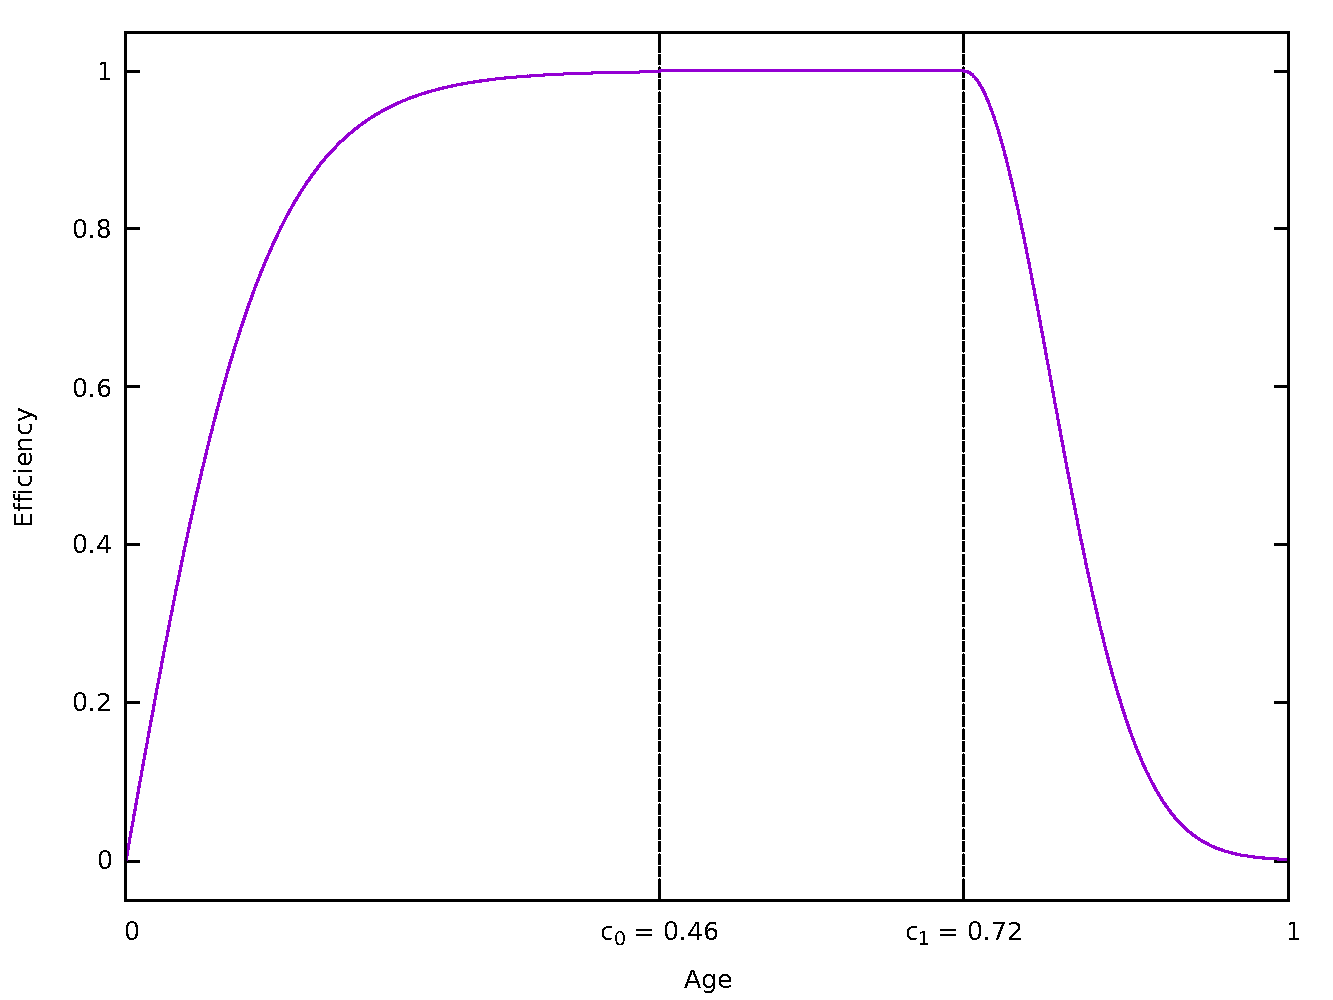
\includegraphics[height=.59\textheight]{efficiency_plot}
 \end{minipage}
 \begin{minipage}{.39\textwidth}
  Age conditions life-step:
  \begin{itemize}
   \item $[0,c_0]$ youth
   \item $[c_0,c_1]$ maturity
   \item $[c_1, 1]$ old age
  \end{itemize}
 \end{minipage}
\end{frame}

\subsubsection{Youth}
\begin{frame}[ok]
 \foreach \i in {0,...,4} {
  \begin{minipage}[c]{.18\textwidth}
   \centering
   \splinoid[scale=.047]{growth_\i}
  \end{minipage}
 }
 \foreach \i in {0,...,4} {
  \begin{minipage}[c]{.18\textwidth}
   \centering\tiny
   \begin{tabular}{c}
    step \i \\
    eff. \pgfmathsetmacro{\e}{100*\i/4}\e \%
   \end{tabular}
  \end{minipage}
 }
 \vfill
 \begin{itemize}
  \item Progressive growth of body size and artifacts
  \item Initial states are highly vulnerable
 \end{itemize}
\end{frame}

\subsubsection{Maturity}
\begin{frame}[ok]
 \begin{itemize}
  \item Reproductive behavior
  \item Based on energy accumulation\footnote{as in \cite{Pichler2008}}
  \item ANN-controlled decision
  \item Not yet implemented
 \end{itemize}
\end{frame}

\subsubsection{Senescence}
\begin{frame}[ok]
  Reduction of maximal speed
  
  > increased chance of starvation and being preyed upon
\end{frame}

\subsection{Sexual dimorphism}
\begin{frame}[ok]
 \begin{minipage}[c]{.49\textwidth}
  \centering \splinoid[scale=.1]{dimorphism_female}
 \end{minipage}
 \begin{minipage}[c]{.49\textwidth}
  \centering \splinoid[scale=.1]{dimorphism_male}
 \end{minipage}
 \vspace{.5\baselineskip}

 \begin{minipage}[c]{.49\textwidth}
  \centering Female
 \end{minipage}
 \begin{minipage}[c]{.49\textwidth}
  \centering Male
 \end{minipage}
 
 \vfill
 Identical genotype (except gender) \\
 $\rightarrow$ different phenotypes (shapes and colors)
\end{frame}

\subsection{Metabolism}
\begin{frame}
 \begin{itemize}
  \item Energy extracted from plants or corpses
  \item Baseline life cost
  \item Consumed energy returned to the environment
 \end{itemize}
\end{frame}

\subsubsection{Clock speed}
\begin{frame}[ok]
 \begin{itemize}
  \item ANN-controlled value
  \item Genetically controlled bounds 
  \item Impacts:
  \begin{itemize}
   \item Motion speed
   \item Resource absorption
   \item Resource consumption
   \item Regeneration
  \end{itemize}
 \end{itemize}
\end{frame}


\subsection{Neural controller}
\begin{frame}
 \begin{tikzpicture}
  
 \end{tikzpicture}
\end{frame}


\section{Environment}
\begin{frame}
 \centering
 \includegraphics[scale=1]{energy_flow}
\end{frame}

\begin{frame}
 \begin{itemize}
  \item Size
  \item Taurus
  \item Obstacles
  \item Plants
 \end{itemize}

\end{frame}


\setbeamertemplate{frametitle}{}
\doendpages[duration=30 s]{}
% \pageatend

\end{document}
 
